\documentclass[11pt, oneside]{article}   	% use "amsart" instead of "article" for AMSLaTeX format
\usepackage{geometry}                		% See geometry.pdf to learn the layout options. There are lots.
\geometry{letterpaper}                   		% ... or a4paper or a5paper or ... 
%\geometry{landscape}                		% Activate for for rotated page geometry
%\usepackage[parfill]{parskip}    		% Activate to begin paragraphs with an empty line rather than an indent
\usepackage{graphicx}				% Use pdf, png, jpg, or eps� with pdflatex; use eps in DVI mode
								% TeX will automatically convert eps --> pdf in pdflatex		
\usepackage{amssymb}
\usepackage{amsmath}
\usepackage{parskip}

\title{Optimization}
%\author{The Author}
%\section{}
% \subsection*{R code}
\date{}							% Activate to display a given date or no date

\graphicspath{{/Users/telliott_admin/Dropbox/Tex/png/}}

\begin{document}
\maketitle
\Large
%\noindent

A general optimization problem expresses some dependence as a function, e.g. $A=f(x)$, where $f(x)$ is moderately complicated.  We wish to find the value of $x$ that gives a maximum (or a minimum) for $A$, perhaps within some limited domain of $x$, or sometimes over all  possible values of $x$.

Usually, the first part is to construct the function $f(x)$, using some constraint that is given in the problem statement.  Then, the basic method is to find the first derivative $A'$ and set it equal to zero, and solve for $x$.

\subsection*{Rectangular area}

We wish to construct a rectangle with the maximum area \emph{for a fixed perimeter} (without the second statement the area would be infinite).  Let's call the sides $x$ and $y$, and the semi-perimeter $S$ (constant) and so our constraint is that 

\[ S = x + y \]

The area is then
\[ A = xy \]
substitute
\[ A = x (S - x) \]
\[ = Sx - x^2 \]

Take the first derivative and set it equal to zero:
\[ A' = S - 2x = 0 \]
\[ x = \frac{S}{2} = y \]
A square has the maximum area for a given perimeter, as expected.

\subsection*{Three-sided fence}

We wish to build a fence, using an existing building for one of the sides, so we need fencing only on three sides.  The total length of available fencing is 500 ft.  This is the constraint.

\begin{center} 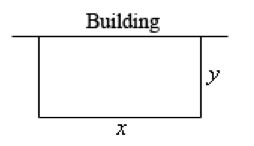
\includegraphics [scale=0.6] {opt1.png} \end{center}

We can use the constraint to express $y$ in terms of $x$:
\[ 500 = 2 y + x \]
\[ y = \frac{500 - x}{2} \]
Now write the area as
\[ A = xy = 250x - \frac{1}{2}x^2 \]
Take the first derivative and set it equal to zero:
\[ A' = 250 - x = 0 \]
Clearly, $x=250$ and $y=125$.

\subsection*{Box with an expensive top}

We wish to build a box.  The box is unusual in that the cost of the top and bottom is more than the sides ($10$ v. $6$ per unit area --- let's say it is in square feet but that doesn't really matter).

\begin{center} 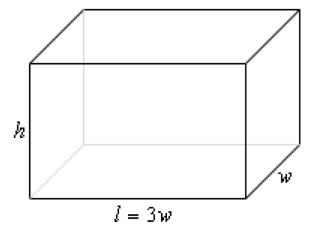
\includegraphics [scale=0.6] {opt2.png} \end{center}

As noted in the figure, the length of the side is three times the width.  We wish to minimize the cost.  

The constraint is that the total volume of the box is $50$ cubic feet.  Using the constraint, we can solve for $h$ in terms of $w$

\[ 50 = 3wwh \]
\[ h = \frac{50}{3w^2} \]

The cost $C$ is
\[ C = 2 \ [ \ 10 \cdot 3w^2 + 6 \cdot wh + 6 \cdot 3 wh \  ] \]
\[ = 2 \ [ 30w^2 + 24wh \  ] \]
\[ = 60w^2 + \frac{800}{w} \]

Take the first derivative and set it equal to zero:
\[ C' = 120 w - \frac{800}{w^2} = 0 \]
\[ w^3 = \frac{800}{120} \]
\[ w = (\frac{800}{120})^{1/3} = 1.88 \]

\subsection*{Box with maximum volume}

This problem features a box with a square base and a total surface area of $S$.  We wish to maximize the volume of the box.

The constraint is the surface area (plus the fact of the square base).  If $b$ is the base length and $h$ is the height, we have that

\[ S = 2b^2 + 4bh \]
\[ h = \frac{S-2b^2}{4b} \]

The volume is
\[ V = b^2 h \]
\[ = b^2 \ \frac{S-2b^2}{4b} \]
\[ = \frac{S}{4} b - \frac{1}{2} b^3 \]

Take the first derivative and set it equal to zero:
\[ V' = \frac{S}{4} - \frac{3}{2}b^2 = 0 \]
\[ S = 6b^2 \]
\[ b = \sqrt{\frac{S}{6}} \]

We can also find $h$
\[ S = 2b^2 + 4bh \]
\[ S = 2\frac{S}{6} + 4h \sqrt{\frac{S}{6}} \]
\[ \frac{1}{3} S = 2h  \sqrt{\frac{S}{6}} \]
\[ h = \frac{1}{\sqrt{6}} \sqrt{S} = b \]

Since $b=h$, what we have is a cube.  Not that surprising. 

\subsection*{Cylindrical can with maximum volume for its surface area}
A cylindrical can is to be formed with a volume of $1.5$ cubic liters.  What are the dimensions if we wish to minimize the surface area (materials used for construction)?

Suppose that the radius is $r$ and the height is $h$.  The formula for volume tells us that
\[ V = 1.5 = \pi r^2 h \]
(Note:  the linear dimensions of this volume, and of $r$,  are in tenths of a meter, since a liter is a cubic decimeter---one-tenth of a meter).

The surface area is 
\[ A = 2 \pi r^2 + 2 \pi r h \]

Substituting for $h$
\[ A = 2 \pi r^2 + 2 \pi r (\frac{1.5}{\pi r^2}) \] 
\[ = 2 \pi r^2 + \frac{3}{r} \] 

Take the first derivative and set equal to zero:

\[ A' = 4 \pi r - \frac{3}{r^2} = 0 \]
\[ r^3 = \frac{3}{4 \pi} \]
\[ r = (\frac{3}{4 \pi})^{1/3} = 0.620 \]
\[ h = \frac{1.5}{\pi r^2}  = 1.24 \]

Multiply by $10$ to get the $r$ and $h$ in centimeters.
\[ r= 6.2 \ \text{cm} \]
\[ h = 12.4 \ \text{cm}  \]

It's no accident that $h = 2r$.

\subsection*{Fancy window}

We wish to construct this window, with a semi-circular arch added on top of the rectangular region below.

\begin{center} 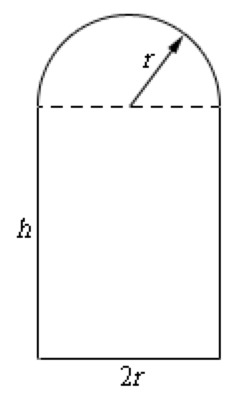
\includegraphics [scale=0.4] {window.png} \end{center}

The quantity to maximize is the area of the window.  The amount of framing for the window is the constraint, with a total length equal to $12$.  Strangely, the framing does not include the dotted line.  Using the constraint, we can solve for $h$ in terms of $r$:
\[ 2h + 2r + \pi r = 12 \]
\[ h = \frac{12 - (2 + \pi) r}{2} \]

The area is 
\[ A = 2rh + \frac{1}{2}\pi r^2 \]
\[ = 12r - (2 + \pi)r^2 + \frac{1}{2} \pi r^2 \]
\[ = 12r - 2r^2 - \frac{1}{2} \pi r^2 \]

We take the first derivative and set it equal to zero:
\[ A' = 12 - 4r - \pi r = 0 \]
\[ r = \frac{12}{4 + \pi} = 1.68 \]
\[ h = \frac{12 - (2 + \pi) r}{2} = 1.68 \]

That's an interesting result!  We should probably revise our drawing, and the client should probably think of a different kind of window.

\subsection*{Projectile range}

Suppose we fire a cannon where the ball has velocity $v$ at an angle $\theta$ with the horizon (straight up would be $\pi/2$ radians).  We wish to determine the angle that will give the maximum range.

This problem has a trick, namely that the distance in the horizontal or $x$-direction depends on the time (and therefore distance) in the $y$-direction, since when $y=0$, the cannonball will fall to earth and not move any more.

If you draw a diagram you will see that 
\[ v_y = v \sin \theta \]
where $v_y$ is the initial velocity in the $y$-direction.

The basic equation of motion under gravity is that 
\[ y = v_y t - \frac{1}{2}gt^2 \]
with $g=32$ so
\[ y = v_y t - 16t^2 \]

At the point of interest $y=0$ so
\[ 0 = v_y t - 16t^2 \]
\[ v_y t = 16 t^2 \]

This has two solutions, namely $t=0$ (not what we are interested in) and
\[ v_y = 16 t \]
\[ t = \frac{v_y}{16} \]
\[ = \frac{v \sin \theta}{16} \]

On the other hand, the quantity we are really interested in is the distance in the $x$-direction.  Similarly to $v_y$, 

\[ v_x = v \cos \theta \]
\[ x = v_x t = v \cos \theta \ \frac{v \sin \theta}{16} \]
\[ = \frac{v^2}{16} \ \cos \theta \sin \theta \]

This looks a little strange but all it really says is that the range is a function of the angle $\theta$ (and also of the square of the velocity).  We take the first derivative and set it equal to zero:

\[ x' = \frac{v^2}{16} \ (\cos^2 \theta - \sin^2 \theta ) = 0 \]

And now we see that the velocity and the gravitational constant will factor out, which makes sense.  It makes intuitive sense that the angle for maximum range (given a velocity), should not depend on that velocity.  We have then that

\[ \cos^2 \theta - \sin^2 \theta = 0 \]
\[ 1 - \sin^2 \theta - \sin^2 \theta = 0 \]
\[ \sin^2 \theta = \frac{1}{2} \]
\[ \sin \theta = \frac{1}{\sqrt{2}} \]
\[ \theta = \frac{\pi}{4} \]

An elevation of $45$ degrees gives the maximum range.

\subsection*{Rectangle in a circle}

Suppose we have a circle of fixed radius $R$, centered at the origin.  Pick a value for $x$ such that $0 \le x \le R$.  Form the rectangle with all four vertices on the circle.  That is, for the $y$ value corresponding to that $x$, the vertices are $\pm \ x, \pm \ y $.

\begin{center} 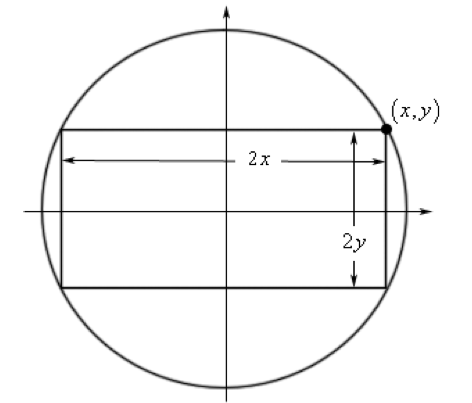
\includegraphics [scale=0.6] {opt3.png} \end{center}

What this means is that given a particular  $x$
\[ y = \sqrt{R^2 - x^2} \]

and therefore the sides of the rectangle are $2x$ and $2\sqrt{R^2 - x^2}$, with area
\[ A = xy = 4x\sqrt{R^2 - x^2} \]

We wish to find the value of $x$ which gives the maximum area.  We will take the first derivative and set it equal to zero.  But, to begin with
\[ \frac{d}{dx} \ \sqrt{R^2 - x^2} = -\frac{1}{2} \frac{2x}{\sqrt{R^2 - x^2}} \]
\[ = -\frac{x}{\sqrt{R^2 - x^2}} \]

so, using the product rule:
\[ A' = (4x)(-\frac{x}{\sqrt{R^2 - x^2}} ) + 4(\sqrt{R^2 - x^2}) = 0 \]
\[ = -\frac{x^2}{\sqrt{R^2 - x^2}} + \sqrt{R^2 - x^2} = 0 \]
\[ x^2 = R^2 - x^2 \]
and since $x^2 + y^2 = R^2$

\[ x^2 = x^2 + y^2 - x^2 = y^2 \]
Thus, $x=y$.  So the maximum area is for a square.  No longer a surprise, I trust.

\subsection*{Closest point to a parabola}

Suppose we consider the simple parabola
\[ y = x^2 \]

Our problem is to find the point(s) $(x,y)$ on the parabola that have the shortest distance to $P=(0,1)$.

One possibility is that $(0,0)$ is the minimum.  But it will turn out that it is not, and so there will be two such points, which are symmetrical about the $y-$axis.  Therefore, we consider only $x \ge 0$.

The distance from any point $(x,y)$ to $P=(0,1)$ is
\[ d = \sqrt{(0-x)^2 + (1-y)^2} \]

It is the case that if we minimize $d^2$, we also minimize $d$, so let's rewrite the equation as

\[ D = (0-x)^2 + (1-y)^2 \]
\[ D = x^2 + 1 - 2y + y^2 \]

Now, the constraint is that $y=x^2$ so plugging in we get

\[ D = y + 1 - 2y + y^2 \]
\[ = 1 - y + y^2 \]

Take the first derivative (with respect to $y$) and set it equal to zero:

\[ D' = -1 + 2y = 0 \]
\[ y = \frac{1}{2} \]
\[ x = \frac{1}{\sqrt{2}} \]

Check the actual distance:

\[ d = \sqrt{(0-x)^2 + (1-y)^2} \]
\[ = \sqrt{(\frac{1}{\sqrt{2}})^2 + (1- \frac{1}{2})^2 } \]
\[ = \sqrt{\frac{1}{2} + \frac{1}{4}} \]
\[ = \frac{\sqrt{3}}{2} \]
\[ = 0.866 \]

\[ (x,y) = (\frac{1}{\sqrt{2}}, \frac{1}{2}) \]

Note that $(1/\sqrt{2},1/2)$ is closer to $(0,1)$ than is $(0,0)$, as we said.

The slope of the line from $(0,1)$ to our point $(1/\sqrt{2},1/2)$ is
\[ \frac{\Delta y}{\Delta x} = \frac{1-1/2}{1/\sqrt{2}} = -\frac{1}{\sqrt{2}} \]

The slope of the tangent to the parabola is $2x$, and at $(1/\sqrt{2},1/2)$ it is

\[ m = 2x = 2 \frac{1}{\sqrt{2}} = \sqrt{2} \]

Since the product of the slopes is $-1$, the line corresponding to the minimum distance is perpendicular to the tangent.


\end{document}  